\chapter{CN-VIP}\label{chap:cn-vip}

\margintoc{}

I already mentioned some of the typing rules related to memory actions and
pointer operations in \nameref{sec:kernel-mem-action-ops}, but I can now
recapitulate them with more detail, drawing special attention to parts about
liveness and bounds checks I skimmed past before. For convenience, I have
reproduced \cref{fig:typing-mem-action} in \cref{fig:cnvip-mem-action}.

\section{Memory actions}

\begin{figure*}[tp]
    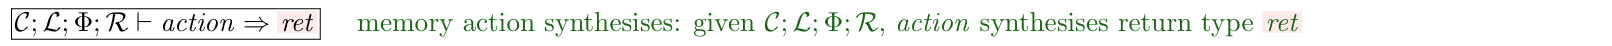
\includegraphics{figures/kernel-mem-action-typing-1}
    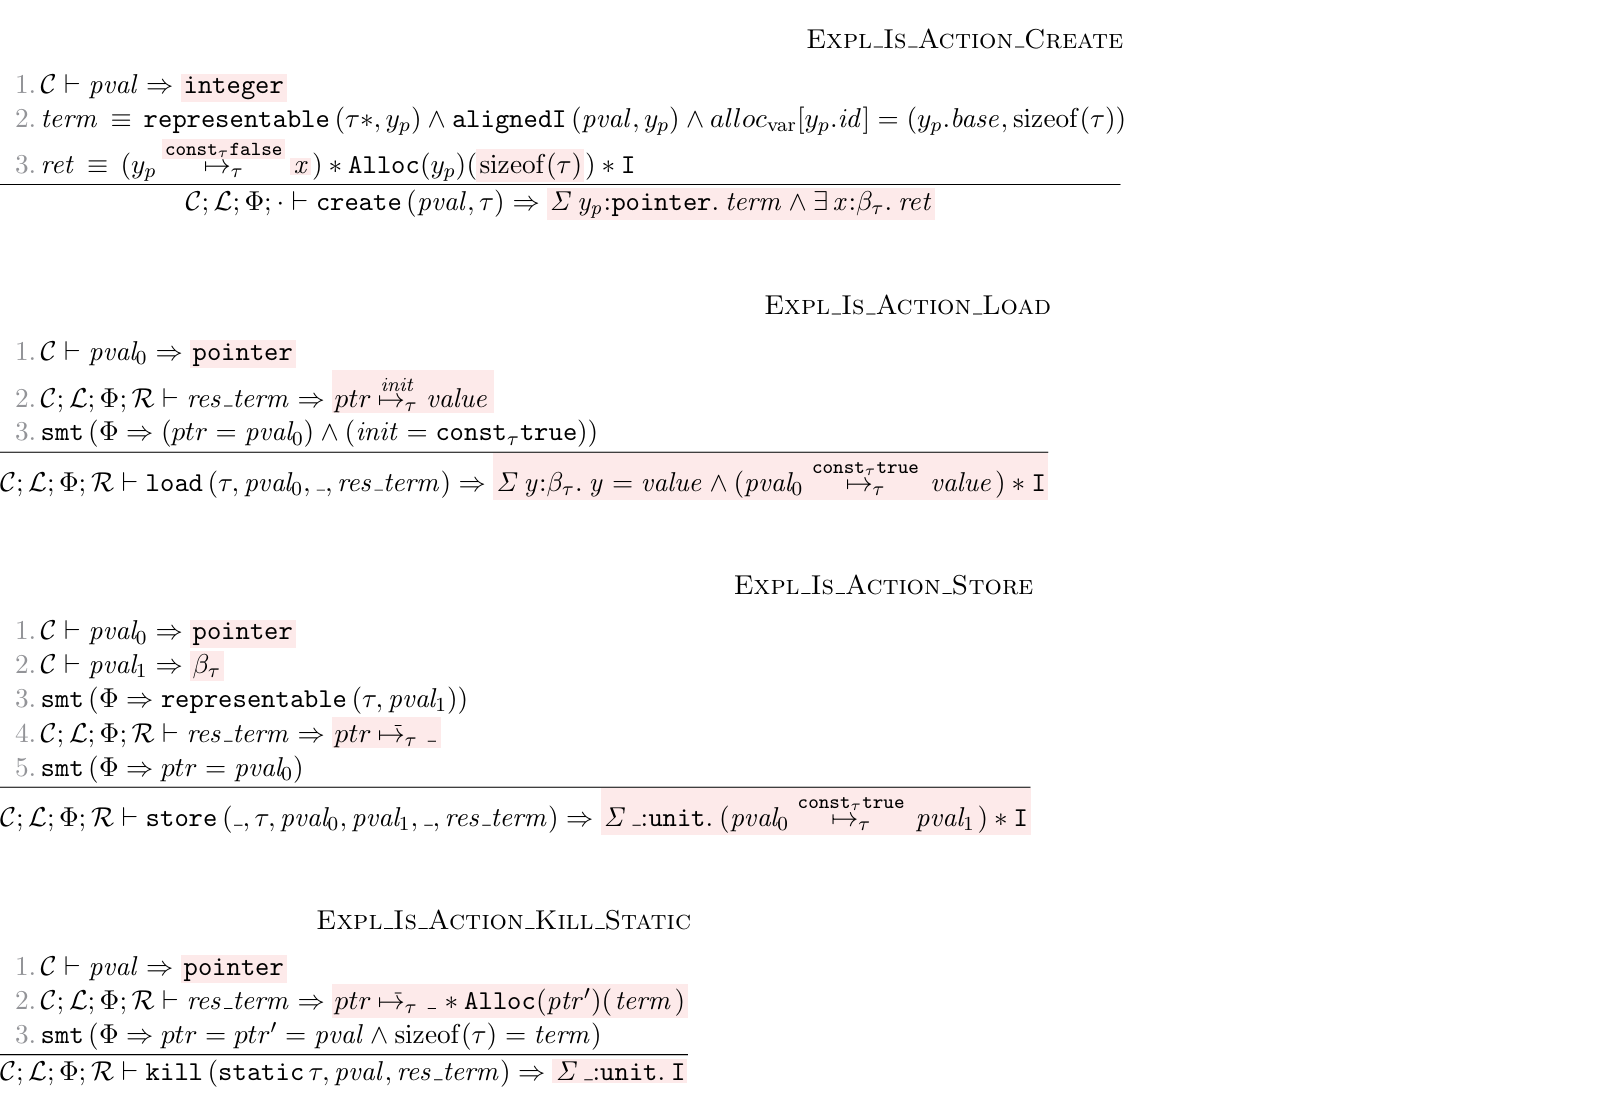
\includegraphics{figures/kernel-mem-action-typing-2}
    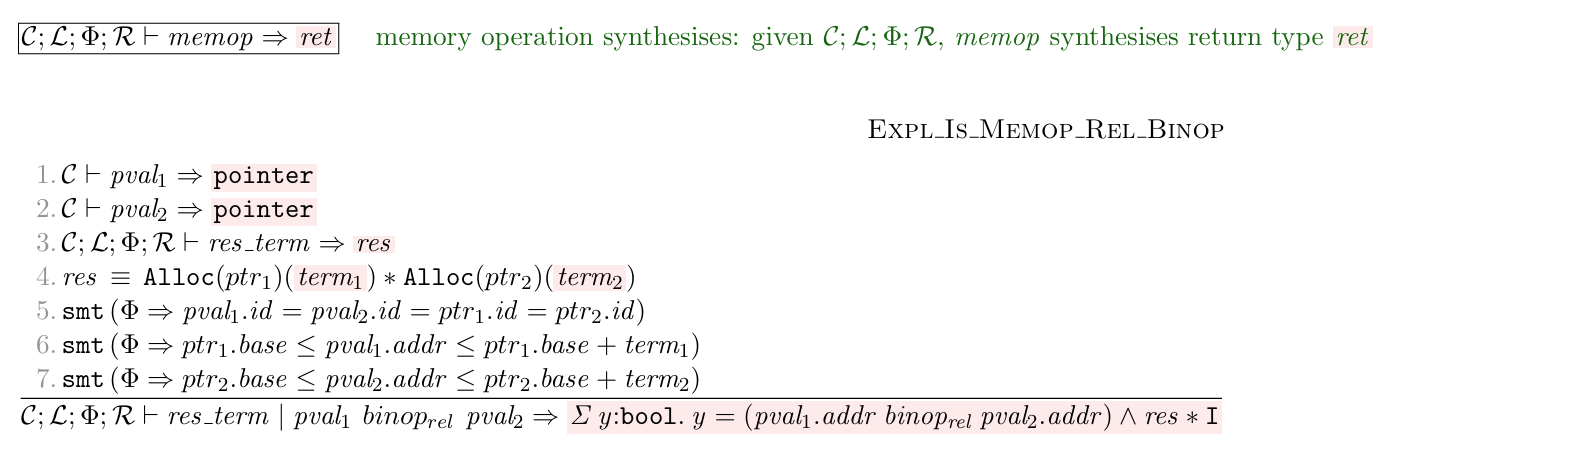
\includegraphics{figures/kernel-memop-typing}
    \caption{\kl{Kernel CN} typing rules for memory actions, and a select rule
        for typing a memory operation.}\label{fig:cnvip-mem-action}
\end{figure*}

In \textsc{Expl\_Is\_Action\_Create}, creating an allocation produces new
constraints on its base address and size. These are tracked via constraints on a
logical variable $\mathit{alloc}_\mathrm{var}$, a map from allocation IDs to
pairs of a base address and size. This can simply be interpreted as an implicit
logical argument and return value for each function call.\sidenote{Need to
check the typing rules to ensure enforce this idea consistently.} Creating an
allocation also produces an \cninline{Alloc} token, to track the fact the
allocation is live, as well as the usual ownership/points-to resource.

TODO\@. Having a memory model also allows me to introduce support for dynamic
memory management. Whereas the above rule is only defined for typed objects
such as locals or globals, a region is essentially just an array of memory
bytes. For simplicity, I model every allocation as succeeding, so that the
pointer returned is never \cinline{NULL}. Hence the typing rule is similar,
but instead of ownership of a single object at a given C type, the ownership
is an iterated one over an array of memory bytes.

Conversely, in \textsc{Exp\_Is\_Action\_Kill}, destroying an allocations
requires both ownership of it (remember ownership represent read/write
permissions, but not allocation and freeing permissions), and the
\cninline{Alloc} token, plus proof that the given pointer is the same as the
owned pointer, and has the same base address as indicated by the allocation
token. For static kills (a block variable going out of scope), the rule also
checks that the size of the C type is also the size of the allocation.
TODO\@. Destroying a region is similar, except with an iterated ownership
of memory bytes.

Fortunately, the rules for loads and stores do not change at all. Ownership of
a location is enough to deduce that the allocation is live, and I assume
ownership is guaranteed to be in bounds for any allocation.\sidenote{Ownership
of out-of-bounds resources is equivalent to $\mathsf{false}$.}

\section{Pointer operations}

There are large discrepancies between the rules for pointer offsets presented
in \sidetextcite{lepigre2022vip} and \sidetextcite{memarian2022cerberus}, and
the \kl{Cerberus source code}, which I have detailed in a table in
\cref{fig:offset-confusion}. I am awaiting clarification on the correct way to
proceed.

\begin{figure*}[tpb]
  \begin{tabular}{ccccc}
  \toprule
   & \citeauthor{lepigre2022vip} incl.\ appendix & \citeauthor{memarian2022cerberus} & Cerberus code \\
  \midrule
  Member (P)
    & {\checksymbol✗}
    & case \cinline{NULL}
    & case \cinline{NULL}, 0-offset
  \\
  Member (ISO)
    & bounds, case 0-offset
    & bounds, liveness
    & case \cinline{NULL}, 0-offset
  \\
  Array (P)
    & {\checksymbol✗}
    & \textendash{}
    & \textendash{}
  \\
  Array (ISO)
    & bounds
    & bounds, liveness
    & bounds, liveness
  \\
  \bottomrule
  \end{tabular}
  \caption{Rules for computing pointer offsets (member and array, with
      pure/permissive (P) and ISO variants) in PNVI-ae-udi, across three
      different sources. `{\checksymbol✗}' means the rule is omitted. `case'
      means the rule special cases on that value. `\textendash{}' means
      there are no checks. `bounds' means a bounds check on the resulting
      pointer. `liveness' means a liveness check on the allocation.}\label{fig:offset-confusion}
\end{figure*}

Pointer operations such as taking the difference between two pointers or
relational comparison between two pointers, require both pointers to be in
bounds of the same live allocation. Hence the rule in\sidenote{TODO fix the
rule, which is very wrong in many ways} \cref{fig:cnvip-mem-action} ask
asks the solver to prove (a) the allocation IDs are equal (b) that the
pointer are within bounds of the allocation (c) to check there exists a
live allocation with that ID\@. The evidence of a live allocation can be
either ownership with the same allocation ID, or an \cninline{Alloc} token,
and the rule is agnostic as to which, just that this evidence is returned
in the type so as to not consume/destroy it.

A rule that is present in the code, but missing in other formats for
\kl{PNVI-ae-udi} is that for casting pointers to dead allocations to integers,
which is permitted so long as the address can fit within the target integer
type. Since \kl{VIP} does not track exposure, the live and the dead
pointer cases collapse into the same case. On top of this, as I mentioned in
\cref{subsec:prov-int-bytes}, I chose to support the limited provenance in
integers required via a new C type, to make the any additional complexity and
performance cost as opt-in, and to avoid changing all the base types for
integers of various sizes (bit vectors) to a datatype with two constructors.
Because of these two simplifications, the cast is therefore just an identity,
on the SMT term and its base type.\sidenote{TODO add this rule} The rules for
casting an integer to a pointer is \kl{UB} if it is not in the \cinline{NULL}
or round-trip case, and is an identity in the latter.\sidenote{TODO add
this rule} And the rule for \cinline{copy_alloc_id} performs a bounds check on
the integer using the allocation ID supplied by the pointer, and combines the
two into a new pointer.\cinline{TODO add this rule too}

The new C types need to be handled with care to implement the subtyping
required for a smoother experience.\sidenote{TODO figure out the subtyping
for base types and resources\ldots}

\section{\cinline{memcpy} and \cinline{memcmp}}

The typing rules for \cinline{memcpy} require iterated ownership of two
contiguous arrays of \kl{memory bytes} of length $n$; it returns ownership of
both, with the constraint that the value of the destination (first) is equal to
that of the source (second). The iterations must be contiguous and of the same
length to express the equality constraint on the values correctly.

The typing rules for \cinline{memcmp} require iterated ownership of two
contiguous arrays of \kl{memory bytes} of length $n$; like \cinline{memcpy}, it
returns ownership of both, unlike \cinline{memcpy} its resulting value is not
straightforward to specify, because the concise or obvious specification would
use quantifiers. I refer to a recursively defined logical function which
constrains the result to be (a) unconstrained if it reads any
\coreinline{unspec} values (b) 0 if all bytes (excluding provenances) are equal
and (c) the difference between the first two unequal bytes otherwise. The presence
of \coreinline{unspec} values makes it difficult to give a simpler specification
to the result such as \cninline[breaklines]{src == dest && result == 0i3 || src
!= dest && result != 0i32}, because we want to do not wish to imply % chktex 26
\cninline{unspec == unspec}.\sidenote{The simpler specification could be
achieved with a notion of \emph{comparable bytes}, converting to which would
require ownership of only initialised and non-padding bytes.}

Both of these typing rules require a way to get ownership of memory bytes, for
which, \kl{CN-VIP} adds new annotations.\sidenote{TODO add these typing rules}
In the formal presentation, these are represented by operations on predicates
which consume ownership of an object, and produce ownership of memory bytes, or
vice versa.

\section{Soundness}\label{sec:cn-vip-soundness}

There are few steps involved to updating the formalisation to use a \kl{VIP}
based memory object model from its current concrete one.
\begin{enumerate}
    \item Extend the configuration of the dynamic semantics to be a step
        relation between abstract \emph{states} and expression, rather than
        just \emph{heaps} and expressions.
    \item Extend the heap typing rules to incorporate the newly added
        allocation history.
    \item Update the proof of soundness for resource term reduction and pattern
        matching, with the new rules.
    \item Define an interpretation of heaps in ResCore, to heaps in the CN-VIP
        memory model.
    \item Prove that the ResCore model of heaps is sound with respect to
        \kl{PNVI-ae-udi}, perhaps via an intermediate concrete memory model.
\end{enumerate}

\subsection{Extending the dynamic semantics}

In the typing rules, I modelled the allocation history as a single global
logical variable $\mathit{alloc}_\mathrm{var}$. This means that even morally
closed programs have that variable free in explicit logical and resource terms.
At the same time, because the allocation history is extended during the course
of evaluating a \kl{ResCore} program, it is not a term which can be substituted
once at the start of the program and close. Hence, the allocation history must
be threaded through to any part of dynamic semantics which relies on checking
constraints (in the empty context) using the SMT solver. At the point of
calling, the allocation history is substituted in, with the most up to date
information, to check the constraint as a closed term (\cref{fig:mem-model-dyn-smt}).

\begin{marginfigure}
    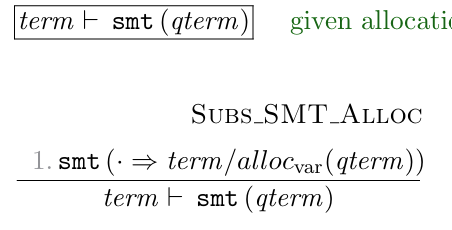
\includegraphics{figures/mem-model-dyn-smt}
    \caption{Calls to the SMT solver are now extended to thread through the
        changing allocation history.}\label{fig:mem-model-dyn-smt}
\end{marginfigure}

Only the \coreinline{create} memory action extends the allocation history, and
so it and every grammar node containing it also includes the allocation history
as part of its configuration, rather than threaded through the
side.\sidenote{TODO fix premise 7 of the create dynamic rules.} Note that
because I split the intuitionistic part of the allocation history from the
linear part, it does not get updated to record a dead allocation in the
rule for \coreinline{kill} (\cref{fig:mem-model-dyn-create-kill}).

\begin{figure*}
    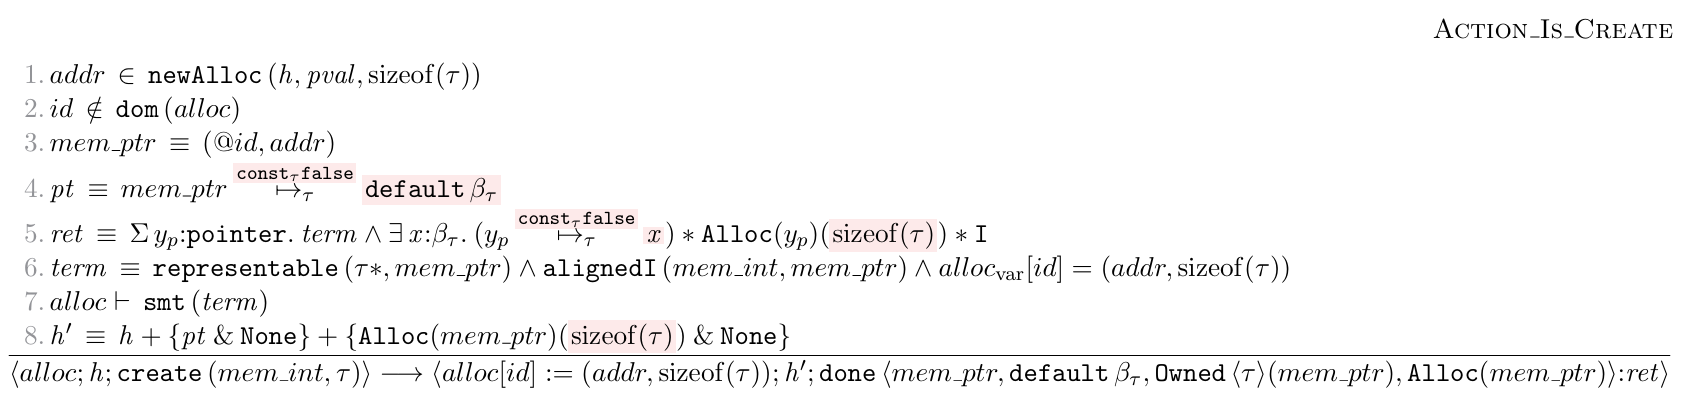
\includegraphics{figures/mem-model-dyn-create}
    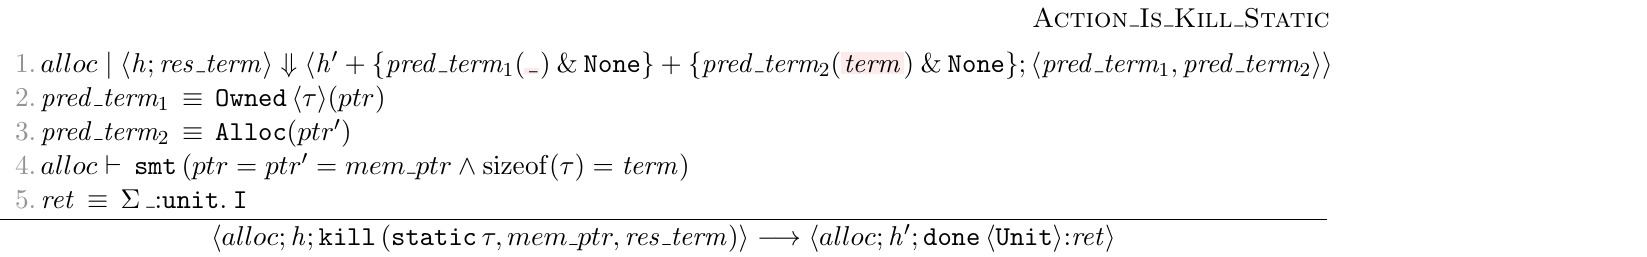
\includegraphics{figures/mem-model-dyn-kill}
    \caption{The allocation history only tracks a mapping from IDs to a pair of
        base address and size, so when an allocation is killed, existing entries
        are not mutated.}\label{fig:mem-model-dyn-create-kill}
\end{figure*}

With the exception of threading through the allocation history, the rules for
loads and stores are unchanged. The rules for converting ownership of objects
into iterated ownership of memory bytes and vice versa are predicate
operations, much like the ones for manipulating structs and fixed-length
arrays.\sidenote{TODO add them} The rules for \coreinline{memcpy} and
\coreinline{memcmp} are also as expected.\sidenote{TODO add them}

Pointer operations do not extend the allocation history, but do require the
heap to check whether the supplied pointers belong to live allocations. They
are agnostic of whether it is ownership or an \cninline{Alloc} token is
provided as evidence (\cref{fig:mem-model-dyn-ptr-relop}).\sidenote{TODO
add/fix this}

\begin{figure*}
    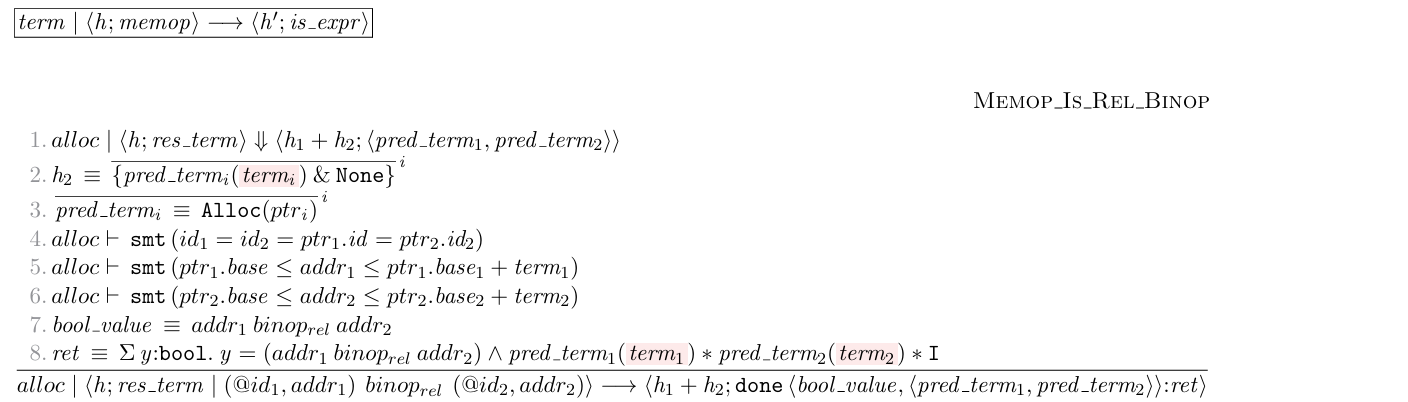
\includegraphics{figures/mem-model-dyn-ptr-relop}
    \caption{Memory operations involving pointers perform a bounds check using
        the SMT solver and supplied pointers, and a liveness check based on
        evidence from the supplied resource term and the heap.}\label{fig:mem-model-dyn-ptr-relop}
\end{figure*}

Lastly, there are the rules about pointer to integer casts, integer to pointer
casts and the \cinline{copy_alloc_id} primitive. The latter two check that that
resulting pointer is in the bounds of a live allocation; they are also agnostic
as to whether it is ownership or an \cninline{Alloc} token which is provided as
evidence.\sidenote{TODO this too\ldots}

\subsection{State typing}

Because the abstract state now includes an append-only allocation history, the
typing rules for heaps (\cref{sec:heap-types}) needs to be generalised to
include it. The main judgement involved in this is $\mathit{alloc} \Leftarrow
\Phi$, which says that the allocation history $\mathit{alloc}$ is consistent
with constraint context $\Phi$. \cref{fig:alloc-typing} shows that it does so
by checking if each constraint, with the allocation history substituted for the
$\mathit{alloc}_\mathrm{var}$, holds (under the empty context).

\begin{marginfigure}
    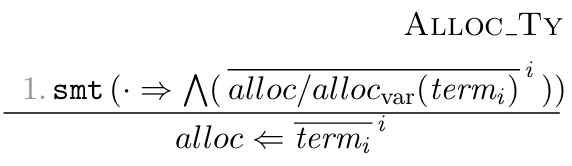
\includegraphics{figures/alloc-typing}
    \caption{Definition of a well-constrained allocation history \textemdash{}
        $\mathit{alloc}$ is consistent with each constraint in context
        $\Phi$.}\label{fig:alloc-typing}
\end{marginfigure}

The heap typing rule generalises similarly (\cref{fig:heap2-typing}). It
substitutes the allocation history for $\mathit{alloc}_\mathrm{var}$, and then
types the heap exactly as before.

\begin{marginfigure}
    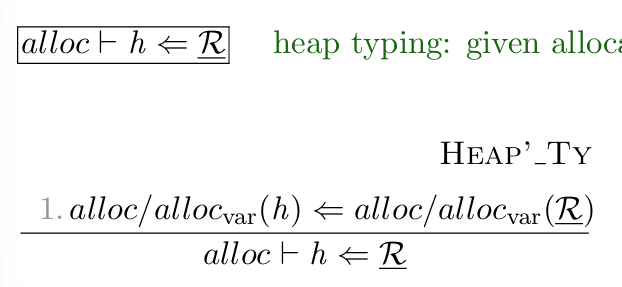
\includegraphics{figures/heap2-typing}
    \caption{Definition of heap typing in the presence of a allocation history:
        substitute the history into the heap and the type (\kl{normalised}
        resource context) and type as before.}\label{fig:heap2-typing}
\end{marginfigure}

\subsection{Updating the soundness proof}

Recall that I defined resource term reduction and pattern matching in the
dynamic semantics in a big-step style (\cref{sec:heap-types}). Whilst this
intertwines the proofs for progress and type preservation, its advantage of
modularity pays off now. The new constructs such as \cinline{memcpy},
\cinline{memcmp}\cinline{copy_alloc_id}, and the conversions to and from memory
bytes, are just additional cases in the proof, the rest are merely updates. The
updates are small because the additional the additional constraints on the
allocation history are easy to link across the static and dynamic semantics by
the definition of allocation history typing. The bounds and liveness checks are
similarly easy to link across the static and dynamic semantics by the
definition of heap typing.

\section{Implementation}

Performance graph

\begin{figure}[h]
    \centering
    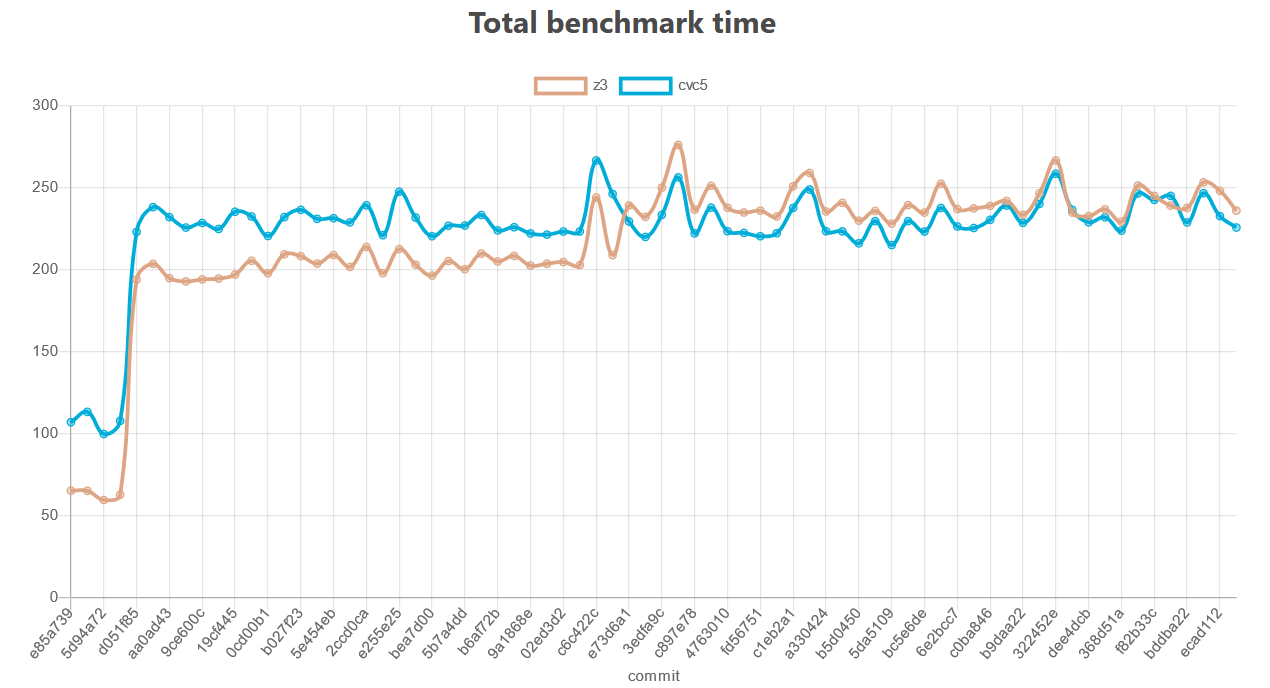
\includegraphics[width=\textwidth]{../misc/vip-performance-hit.png}
\end{figure}

\url{https://rems-project.githb.io/cerberus/dev/bench/}

\section{Translating resource lemmas}\label{sec:trans-res-lemmas}

Is there a reason, in the discussion about Cassia's PhD, we thought all of
Cerberus needed to be shoved into Iris instead of just a trace of memory model
(and eventually, concurrency) events?

irisification (cf
\url{https://people.mpi-sws.org/~dreyer/papers/iris-ground-up/paper.pdf}).  Either
just the resource algebra or (as DM suggests) also the abstract language of
memory model interface events: which one let one formalise the primitive
resource-context manipulations that CN does (conceivably extractably).

I think a sufficient halfway point would be the language of traces memory
events i.e.\ memory model as the dynamics. Resource algebra would be CN's view
of resources. Resource lemmas are then just statements saying that one resource
represents exactly the same heap as another resource (skips). Changes to the
resource algebra because of memory events (which we could introduce unsoundness
in CN) would be proved sound in Iris.

As a bonus, we could even formalise and prove sounds the inference procedures
CN uses (and with some engineering to handle SMT, even extract from Rocq).

The inference I'm talking about is resource context manipulations: checking if
we can pack or unpack predicates, if an owned is in the context, shifting
indices in and out of iterated predicates, exploding and imploding structs.
These operations don't require core structure.

Even if full extraction of the inference algo is not feasible (it would
involves standard data structures + SMT FFI), having a defined set of resource
manipulation primitives proved sound and extracting those (just standard data
structure manipulations), or even just proving the primitives sound and using a
similar interface would increase confidence.

If ones reads the above in reverse, it even provides a gradual migration path
which doesn't commit us to any next step and allows us to see how far
extraction can take us.

If the inference algs or the primitives are formalised, then we can iterate on
cleverer  inference schemes with a strong safety net

I think it will become more valuable as soon as we start having fancier things
like higher-order resources, locks, fractional permissions. At that point,
checking the steps/moves that any inference algorithm could take would get
closer to essential.

Even if an arbitrary inference algorithm is not stable, the steps available and
the shape of the resources should be more so, and that is worth at least
creating a clean abstraction for (and then pen-paper soundness, and then
mechanised soundness).

Noted and agreed that anything mechanised takes longer than one wants/expects
and that extraction is a pain. But this gives us a concrete use-case,
reasonable sequence of experiments and a clear idea of the benefits and costs.

